%================================================================
\section{Teori}\label{sec:Teori}
%================================================================

%----------------------------------------------------------------
\subsection{Prosjekt teori 1}\label{sec:prosjekt teori}
%----------------------------------------------------------------
Dette er \autoref{sec:prosjekt teori}.

Kildehenvisning gjøres med \hologo{BibTeX} \cite[s.~100]{Sakurai}.

Kryssreferer ligninger som
\begin{equation}\label{eq:einstein}
    E = m c^2
\end{equation}
med \cref{eq:einstein}.

\autoref{fig:glad} viser et lykkelig dyr. 
\begin{figure}[H]
\begin{center}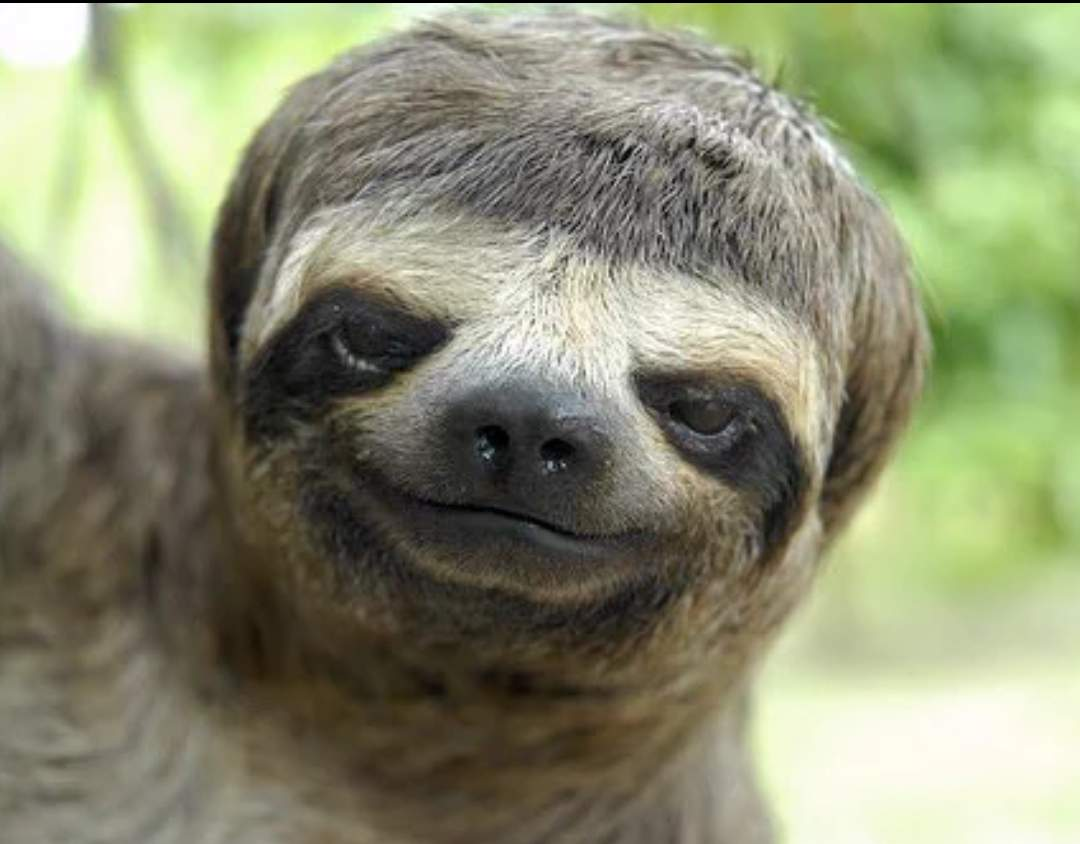
\includegraphics[scale=0.5]{Figures/Funny-Animal-Face.jpg}
\end{center}
\caption{Dovendyr er trelevende pattedyr kjent for sin treghet og for å vie det meste av sine liv til å henge opp ned i trær.}
\label{fig:glad}
\end{figure}

\autoref{tab:skiftende} lister opp noen verdier med skiftende farge på radene. 
\begin{table}[H]
\caption{Skiftende bakgrunnsfarge på radene.}
\centering
\rowcolors{2}{gray!25}{white}
\begin{tabular}{ccc}
\hline
\hline 
$\alpha$ & $\beta$ & $\gamma$
\\
\hline 
\hline 
0.1 & 0.2 & 0.3
\\
0.4 & 0.5 & 0.6
\\
0.7 & 0.8 & 0.9
\\
\hline
\end{tabular}
\label{tab:skiftende}
\end{table}
